\documentclass[11pt,a4paper]{article}

\usepackage[T1]{fontenc}
\usepackage[utf8]{inputenc}
\usepackage{lmodern}
\usepackage[margin=2.4cm]{geometry}
\usepackage{microtype}
\usepackage{booktabs}
\usepackage{multirow}
\usepackage{graphicx}
\usepackage{float}
\usepackage{subcaption}
\usepackage{amsmath}
\usepackage{amssymb}
\usepackage{siunitx}
\usepackage[dvipsnames]{xcolor}
\usepackage{tikz}
\usetikzlibrary{positioning,arrows.meta,decorations.pathreplacing,fit,backgrounds}
\usepackage[colorlinks=true,allcolors=NavyBlue!70!black]{hyperref}

\sisetup{detect-all, group-minimum-digits=4, group-digits=integer}
\setlength{\emergencystretch}{3em}

\newcommand{\rmse}{nRMSE}
\newcommand{\best}[1]{\textbf{#1}}
\newcommand{\reportone}{Report~I}
\newcommand{\reporttwo}{Report~II}
\newcommand{\fals}{\textit{Falsifier.}\ }

\title{\bfseries MRIxFields 2026: Research Plan\\[0.3em]
\large Two Horizons: Challenge Submission and Continuation}
\author{Berkin Deniz Kahya \and Furkan Yüceyalç\i{}n \and Racha Badreddine \and Ahmet Zelka}
\date{}

\begin{document}
\maketitle

\begin{abstract}
\noindent
This document is the explainer for the working plan: for each item, what changes in the code, why the
log justifies it, and what result would falsify it. \textbf{SSIM is the metric we are ranked on}, so it
is the metric the position table is sorted by and the one every comparison below leads with. Four
measured facts set the priorities. First, six weeks of architecture search have bought
\num{+0.0012} SSIM: the original conditional U-Net of 18 July scored \num{0.9014}, and FPS-Former,
Swin~UNETR, the tubelet LeJEPA encoder and a 3D U-Net have since produced \num{0.9026}, with the top four
entries inside \num{0.005} SSIM of one another and no seed-noise floor measured. Second, the August
rebuilds of that same conditional U-Net \emph{regressed}, to \num{0.8976} at 50 epochs and \num{0.8986},
both below the July 10-epoch original; and there is an unmonitored mechanism for exactly that, since the
2D configurations define no validation split, so early stopping watches \emph{training} loss and
``restore best'' restores the most overfit weights. Third, conditioning remains the only large measured
effect, \num{0.8699} unconditioned against \num{0.8976} conditioned. Fourth, the July checkpoint is
unrecoverable: only its submission ID survives, so that number can be re-earned but not re-derived. The
plan follows. Horizon~A builds a held-out fold, re-reads the six checkpoints already on disk before
training anything new, takes the free SSIM, submits a zero-parameter calibration control, and spends its
remaining budget on conditioning and on one matched encoder control. The tubelet encoder question is
\emph{unresolved rather than settled}: at a matched two-epoch budget the LeJEPA initialisation wins
\rmse{} and LPIPS and loses SSIM by \num{0.0049}, which is inside the unmeasured seed spread, and the
pretraining monitor's dense-token collapse is measured on the encoder's final layer --- which is not the
layer the translator reads.
\end{abstract}

\section{Position}
\label{sec:position}

Table~\ref{tab:position} is the Task~3 log, modality-averaged, sorted by SSIM.

\begin{table}[H]
  \centering
  \small
  \caption{Task~3, modality-averaged, sorted by the ranked metric. The runs differ in budget and in
  dimensionality, so no row pair here is controlled except the unconditioned/conditioned one. INPUT is
  the unmodified input submitted as its own prediction.}
  \label{tab:position}
  \begin{tabular}{lccclc}
    \toprule
    Model & SSIM~$\uparrow$ & \rmse{}~$\downarrow$ & LPIPS~$\downarrow$ & Experiment & Date \\
    \midrule
    \best{UNet-3D} & \best{0.9026} & \best{0.2329} & \best{0.0816} & \best{3D U-Net, 10 ep} & \best{02/09} \\
    \best{UNet}    & \best{0.9014} & 0.2364 & 0.0890 & \best{``New baseline?'', original, 10 ep} & \best{18/07} \\
    UNet           & 0.8986 & 0.2336 & 0.0819 & conditioned (Furkan) & 30/08 \\
    UNet           & 0.8976 & 0.2412 & 0.0895 & conditioned, 50 ep & 30/08 \\
    UNet-3D        & 0.8942 & 0.2436 & 0.0967 & 3D U-Net, 2 ep & 31/08 \\
    UNet-3D        & 0.8893 & 0.2383 & 0.0889 & tubelet LeJEPA encoder, 2 ep & 29/08 \\
    FPS-Former     & 0.8795 & 0.2471 & 0.1492 & 203 ep & 02/09 \\
    UNet           & 0.8699 & 0.4022 & 0.1198 & unconditioned & 30/08 \\
    INPUT          & 0.8365 & 0.5216 & 0.1573 & source control (zero point) & 28/08 \\
    Swin UNETR 3D  & 0.8315 & 0.3002 & 0.1713 & 10 ep & 31/08 \\
    StarGAN~v2     & 0.7397 & 0.3436 & 0.1545 & challenge baseline & 15/07 \\
    \bottomrule
  \end{tabular}
\end{table}

\paragraph{1. Six weeks of architecture search has bought \texorpdfstring{$+0.0012$}{+0.0012} SSIM.} The
July model scored \num{0.9014}; FPS-Former~\cite{meng2025fpsformer}, Swin~UNETR, the tubelet LeJEPA
encoder and the 3D U-Net have since produced \num{0.9026}. The top four rows sit inside \num{0.005} SSIM of each other and
\emph{nobody has measured the seed-noise floor}, so it is not established that they differ at all.

\paragraph{2. The re-implementations regressed.} The same conditional-U-Net idea, rebuilt in August,
scores \num{0.8976} at 50 epochs and \num{0.8986} --- both below the July 10-epoch original. More
training, worse SSIM.

\paragraph{3. There is a mechanism for that, and it is unmonitored.}
The 2D training configuration sets \texttt{epochs = 100} with
\texttt{early\_stopping\_patience = 10} and \texttt{early\_stopping\_restore\_best = true}, and defines no
validation or holdout keys at all (\texttt{configs/task3\_unet\_pro.toml}). So \texttt{validation\_loader is None},
\texttt{components/training/task3.py:228} falls back to monitoring \emph{training} loss, and
``restore best'' then restores the best training loss, i.e.\ the most overfit weights. That run reached
at least epoch 60: \texttt{runs/task3\_unet\_pro/artifacts/} holds epochs 10 through 60.

\paragraph{4. Conditioning remains the only large measured effect.} Unconditioned \num{0.8699} against
conditioned \num{0.8976} SSIM at matched settings, a clean ablation because
\texttt{UnconditionalUNet} is the same architecture minus two embeddings.

\paragraph{The July model cannot be recovered.} No artifacts exist before 2026-08-30 in
\texttt{OUTPUT\_DIR} or \texttt{experiment-pipeline/runs/}; mlflow's earliest run is 2026-08-30; this
repository's first commit is 2026-08-06. Only submission ID \num{9772388} survives, so that number can
be re-earned but not re-derived. The reading that follows: a substantial part of the last six weeks may
have been resolving checkpoint-selection noise rather than architecture. That is cheap to test, and the
test comes first.

\section{Horizon A --- the challenge submission}
\label{sec:horizonA}

Twelve days. The rule for admission is cheap and high certainty: no new architecture, and no item whose
payoff depends on an untested premise.

\subsection{A0 --- instrument, then read the checkpoints we already have}
\label{sec:A0}

We are chasing SSIM differences of about \num{0.005} with no local held-out signal, on models whose early
stopping watches training loss. Four runs under those conditions produce four numbers that cannot be
ordered.

\paragraph{A0.1 --- give the 2D data module a held-out subject.}
\texttt{components/data/task3.py:55} returns only \texttt{\{"train", "pretrain"\}}; there is no
validation split anywhere in the 2D path. The volumetric module
(\texttt{components/data/\allowbreak task3\_volume.py}) already implements \texttt{holdout\_subjects}, and
the Swin configuration (\texttt{configs/\allowbreak task3\_swin\_unetr\_pro.toml:37}) already uses it with
\texttt{["0009"]}. Port the mechanism. Subjects \texttt{0006}, \texttt{0007}, \texttt{0009} give three
folds. Nothing else in A0--A5 is interpretable without it.
\fals If the held-out SSIM ordering of configurations we have already submitted disagrees with their
leaderboard ordering, the local instrument is not measuring the scored quantity and must not be used to
select submissions.

\paragraph{A0.2 --- report per transition \texorpdfstring{$\times$}{x} per modality.} Twenty transitions
whose $\Delta\alpha$ differs by an order of magnitude are collapsed into one scalar. A model that works
at \SI{0.1}{\tesla} and one that copies at \SI{5}{\tesla} are indistinguishable in today's readout, and
\reportone{} showed copying scores well --- the identity control's SSIM \num{0.8365} is within
\num{0.07} of the leader.
\fals If the leader's per-transition SSIM profile is flat across $\Delta\alpha$, the transitions are
behaving interchangeably and the physics conditioning of A3.2 and the spectral loss of B5 lose their
motivation.

\paragraph{A0.3 --- seed-noise floor.} Run the current best configuration twice with different seeds.
Given that the top four models span \num{0.005} SSIM, this is not a formality: it is the item that
decides whether Table~\ref{tab:position} can be read at the resolution we have been reading it at.
\fals If the seed spread exceeds \num{0.005} SSIM, then no ordering among the top four rows is
established, the \num{0.0049} SSIM gap that currently demotes the encoder (A5.2) is not a result either,
and every later comparison needs multiple seeds or must be abandoned.

\paragraph{A0.5 --- sweep the checkpoints already on disk. No training required.} Six of them are
already there. The directory \texttt{runs/task3\_unet\_pro/artifacts/} holds epochs 10, 20, 30, 40, 50
and 60 of the run behind the August rows. Score all six on the held-out fold, SSIM primary, per
transition. This is the direct test of
conclusion~3: the selected weights are the most overfit ones available, so if held-out SSIM peaks near
epoch 10 and decays, the July result and the August regression have one explanation between them, and
checkpoint selection is worth more SSIM than any architecture tried since. Hours of compute, no
training, and it decides what A1--A5 are for.
\fals If held-out SSIM is flat or rising in epoch across the six checkpoints, checkpoint selection is
not the explanation, the July-to-August gap needs a different one, and the architecture comparisons in
Table~\ref{tab:position} stand as run.

\paragraph{A0.4 --- early stopping on the held-out fold.} Once A0.1 lands, the 2D configurations can
set \texttt{early\_stopping\_monitor = "validation"}, as \texttt{task3\_tubelet\_pro.toml} already does.
\fals If the best held-out epoch is the last epoch in all three folds, there is no overfitting to catch
at these budgets, A0.5 will come back flat, and the budget question is under-training instead.

\subsection{A1 --- free wins on the current best model}
\label{sec:A1}

None of these needs a new architecture and all are near-zero risk. All three act on SSIM specifically.

\paragraph{A1.1 --- predict the residual, not the image.} The 2D head is
\texttt{Conv2d(...,1) $\to$ Tanh} (\texttt{components/models/conditional\_unet.py:59}), so the network
reconstructs the entire image through a saturating nonlinearity while the identity control already scores
SSIM \num{0.8365}. Switch to $\mathrm{out} = x + f(x)$ with a zero-initialised head
(Figure~\ref{fig:head}). The pattern is already in the repository, in logit space, in the tubelet
consumer (\texttt{lejepa\_pretraining/\allowbreak repo/\allowbreak mrixfields\_downstream/\allowbreak tubelet\_model.py:236--239}:
$\mathrm{sigmoid}(\mathrm{logit}(x) + r)$); port it rather than inventing one. SSIM is a structural
metric and the source structure is exactly what the current head throws away and re-earns.
\fals If the residual head matches the current head on held-out SSIM within the A0.3 seed floor on all
three folds, the network was not paying a measurable price for rebuilding structure it was handed.

\paragraph{A1.2 --- eight-way dihedral test-time augmentation.} Flips $\times$ \texttt{rot90}, averaged
at inference. It appears nowhere in the log. No training cost.
\fals Averaging is a smoothing operation: if it raises SSIM but degrades LPIPS, the rank-sum trade can be
negative, so all three metrics must be read before a submission slot is spent.

\paragraph{A1.3 --- checkpoint weight averaging} over the artifacts already sitting in the run
directories, \texttt{experiment-pipeline/runs/*/artifacts/}, which costs one evaluation pass and no
training. A0.5 supplies the per-epoch held-out curve that says which checkpoints are worth averaging.
\fals If the averaged weights score worse than the best single checkpoint on the held-out fold, the
checkpoints are not from one basin --- different runs or schedules --- and the item is inapplicable.

\paragraph{A1.4 --- submit the best combination} of A1.1--A1.3.
\fals If the combination underperforms the best single component locally, the components interact and
the submission should carry the single component instead.

\begin{figure}[t]
  \centering
  \resizebox{0.62\linewidth}{!}{%
  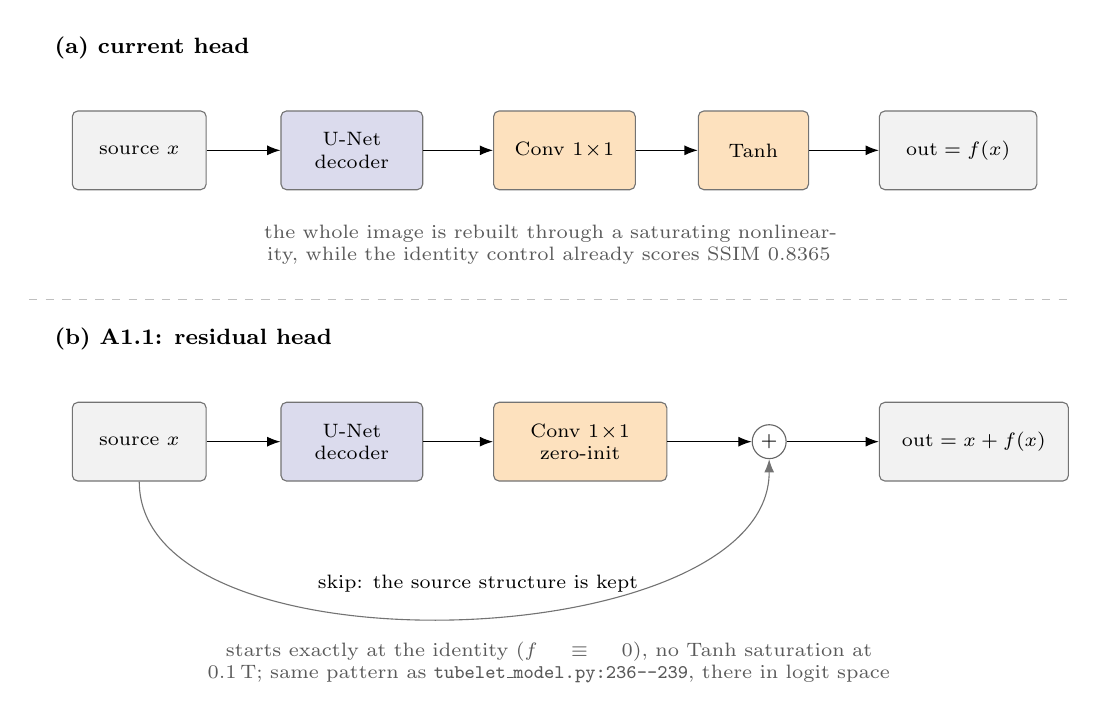
\begin{tikzpicture}[
    >=Latex,
    font=\small,
    blk/.style={draw=black!55, rounded corners=2pt, minimum height=10mm, align=center, font=\scriptsize},
    gen/.style={blk, fill=black!5},
    act/.style={blk, fill=BurntOrange!22},
    net/.style={blk, fill=NavyBlue!14},
  ]
    % ---------- (a) ----------
    \node[font=\bfseries\footnotesize, anchor=west] at (-0.6,1.3) {(a) current head};
    \node[gen, minimum width=17mm] (x)  at (0.6,0)  {source $x$};
    \node[net, minimum width=18mm] (u)  at (3.3,0)  {U-Net\\decoder};
    \node[act, minimum width=18mm] (c)  at (6.0,0)  {Conv $1\!\times\!1$};
    \node[act, minimum width=14mm] (t)  at (8.4,0)  {Tanh};
    \node[gen, minimum width=20mm] (o)  at (11.0,0) {$\mathrm{out}=f(x)$};
    \foreach \a/\b in {x/u, u/c, c/t, t/o} \draw[->] (\a) -- (\b);
    \node[font=\scriptsize, align=center, text width=125mm, black!65] at (5.8,-1.2)
      {the whole image is rebuilt through a saturating nonlinearity, while the identity control
       already scores SSIM \num{0.8365}};

    \draw[black!25, dashed] (-0.8,-1.9) -- (12.4,-1.9);

    % ---------- (b) ----------
    \node[font=\bfseries\footnotesize, anchor=west] at (-0.6,-2.4) {(b) A1.1: residual head};
    \node[gen, minimum width=17mm] (x2) at (0.6,-3.7)  {source $x$};
    \node[net, minimum width=18mm] (u2) at (3.3,-3.7)  {U-Net\\decoder};
    \node[act, minimum width=22mm] (c2) at (6.2,-3.7)  {Conv $1\!\times\!1$\\zero-init};
    \node[circle, draw=black!60, inner sep=1.5pt, font=\scriptsize] (s2) at (8.6,-3.7) {$+$};
    \node[gen, minimum width=24mm] (o2) at (11.2,-3.7) {$\mathrm{out}=x+f(x)$};
    \foreach \a/\b in {x2/u2, u2/c2, c2/s2, s2/o2} \draw[->] (\a) -- (\b);
    \draw[->, black!55] (x2.south) to[out=-90, in=-90, looseness=0.8] (s2.south);
    \node[font=\scriptsize, black] at (4.9,-5.5) {skip: the source structure is kept};
    \node[font=\scriptsize, align=center, text width=130mm, black!65] at (5.8,-6.5)
      {starts exactly at the identity ($f \equiv 0$), no Tanh saturation at \SI{0.1}{\tesla}; same
       pattern as \texttt{tubelet\_model.py:236--239}, there in logit space};
  \end{tikzpicture}}
  \caption{A1.1. The current head reconstructs the target from scratch and must re-earn the structure the
  source already supplies; the residual head is handed it. The zero-initialised $1\times1$ convolution
  makes the change an initialisation-preserving reparameterisation: (b) starts from the identity
  control's score rather than below it. The tubelet translator of Section~\ref{sec:A5} already has this
  head, in logit space; A1.1 is the 2D leader catching up with it.}
  \label{fig:head}
\end{figure}

\subsection{A2 --- the calibration control}
\label{sec:A2}

\paragraph{A2.1.} Fit the per-(modality, source, target) monotone quantile map of finding~F4 on all three
paired subjects and submit it. Zero parameters, no network, no training, one submission slot, half a day.

F4 measured that this map removes \SI{46}{\percent} of the identity control's error (\num{0.6218} to
\num{0.3358} over twenty transitions, leave-one-subject-out), and F3 measured that the trained U-Net's
target conditioning is \SIrange{12}{96}{\percent} explained by a single global affine. If a
parameter-free histogram match lands near the leader on \rmse{}, a large part of what
Table~\ref{tab:position} has been resolving is calibration quality. Two caveats keep this at one
submission slot rather than at the top of the plan: F4's local \rmse{} convention,
$\lVert p - t\rVert_2 / \lVert t \rVert_2$ over the target brain mask, is \emph{not} the platform's, so
only the ratio was claimed; and F4 measured \rmse{} only, while the ranked metric is SSIM, on which a
monotone intensity map has no measured effect at all.
\fals If the calibration control lands near the identity control (SSIM \num{0.8365}, \rmse{}
\num{0.5216}) rather than near the U-Net, F4's ratio does not survive the change of normalisation and the
calibration reading is wrong; if it improves \rmse{} but not SSIM, the finding is real and simply does
not touch the metric we are ranked on.

\subsection{A3 --- conditioning, the one lever with headroom}
\label{sec:A3}

\paragraph{A3.1 --- FiLM at every decoder scale.} Today the entire conditioning signal is one broadcast
add at the bottleneck: \texttt{conditional\_unet.py:76--77} computes
\texttt{source\_embedding(d\_src) + target\_embedding(d\_tgt)} and adds it to the \num{512}-channel
bottleneck, after which four decoder stages run with no further reference to the transition
(Figure~\ref{fig:film}a). Replace it with per-scale scale-and-shift after each \texttt{InstanceNorm2d} in
\texttt{\_ConvBlock}, zero-initialised so that $\gamma = 1$, $\beta = 0$ and the model begins numerically
identical to the current one. The block does not need to be written: it exists three times already, as
\texttt{\_ConditionalRefinement} in \texttt{conditional\_swin\_unetr.py:19}, as the adaptive-norm unit in
\texttt{conditional\_vit.py:26}, and --- fully wired, at four decoder stages, zero-initialised --- in the
tubelet translator of Section~\ref{sec:A5}.
\fals If per-scale FiLM matches the single bottleneck add on held-out SSIM within the seed floor, the
constraint is not \emph{where} conditioning enters but \emph{what} it can express, and the effort moves
to A3.2.

\paragraph{A3.2 --- condition on physics, not fifteen opaque indices.} The current embeddings are indexed
by $5m + c$ over three modalities and five fields, so each of the fifteen domains learns its own vector
from three subjects and the twenty transitions share nothing. Feed the physics features
$\big(\text{modality one-hot},\ \log B_0^{\mathrm{src}},$
$\log B_0^{\mathrm{tgt}},\ \Delta\alpha(\mathrm{src}\!\to\!\mathrm{tgt})\big)$ through a small MLP that
produces the FiLM parameters instead (Figure~\ref{fig:film}b). This is constructible today: all
$20 \times 3$ transition-by-modality $\Delta\alpha$ cells resolve in
\texttt{reports/spectral/alpha\_summary.csv} on the retrospective split, 30 volumes each, so no new
measurement is needed. The tubelet translator's conditioning is already halfway there --- three separate
embeddings for source field, target field and modality rather than one fifteen-way index --- but it is
still learned rather than physical.
\fals If the physics parameterisation is worse than free per-domain FiLM embeddings on held-out SSIM, the
transitions do not share the structure these four features encode, and the correct move is the opposite
one: per-transition low-rank adapters on a shared backbone.

\paragraph{A3.3 --- control: delete the source embedding.} F2 measured that changing the declared source
field moves the output by \SIrange{1.1}{2.1}{\percent} of its dynamic range while changing the target
moves it by \SIrange{19.7}{53.7}{\percent}: the trained model is effectively
$f(\text{image}, \text{target})$. Remove \texttt{source\_embedding} and retrain.
\fals Symmetric and informative either way. If removal costs nothing, the model simplifies and F2 is
confirmed under training rather than at one checkpoint. If it costs measurable SSIM, F2 was a
one-checkpoint, one-subject, one-slice measurement that has been over-read.

\begin{figure}[t]
  \centering
  \resizebox{0.78\linewidth}{!}{%
  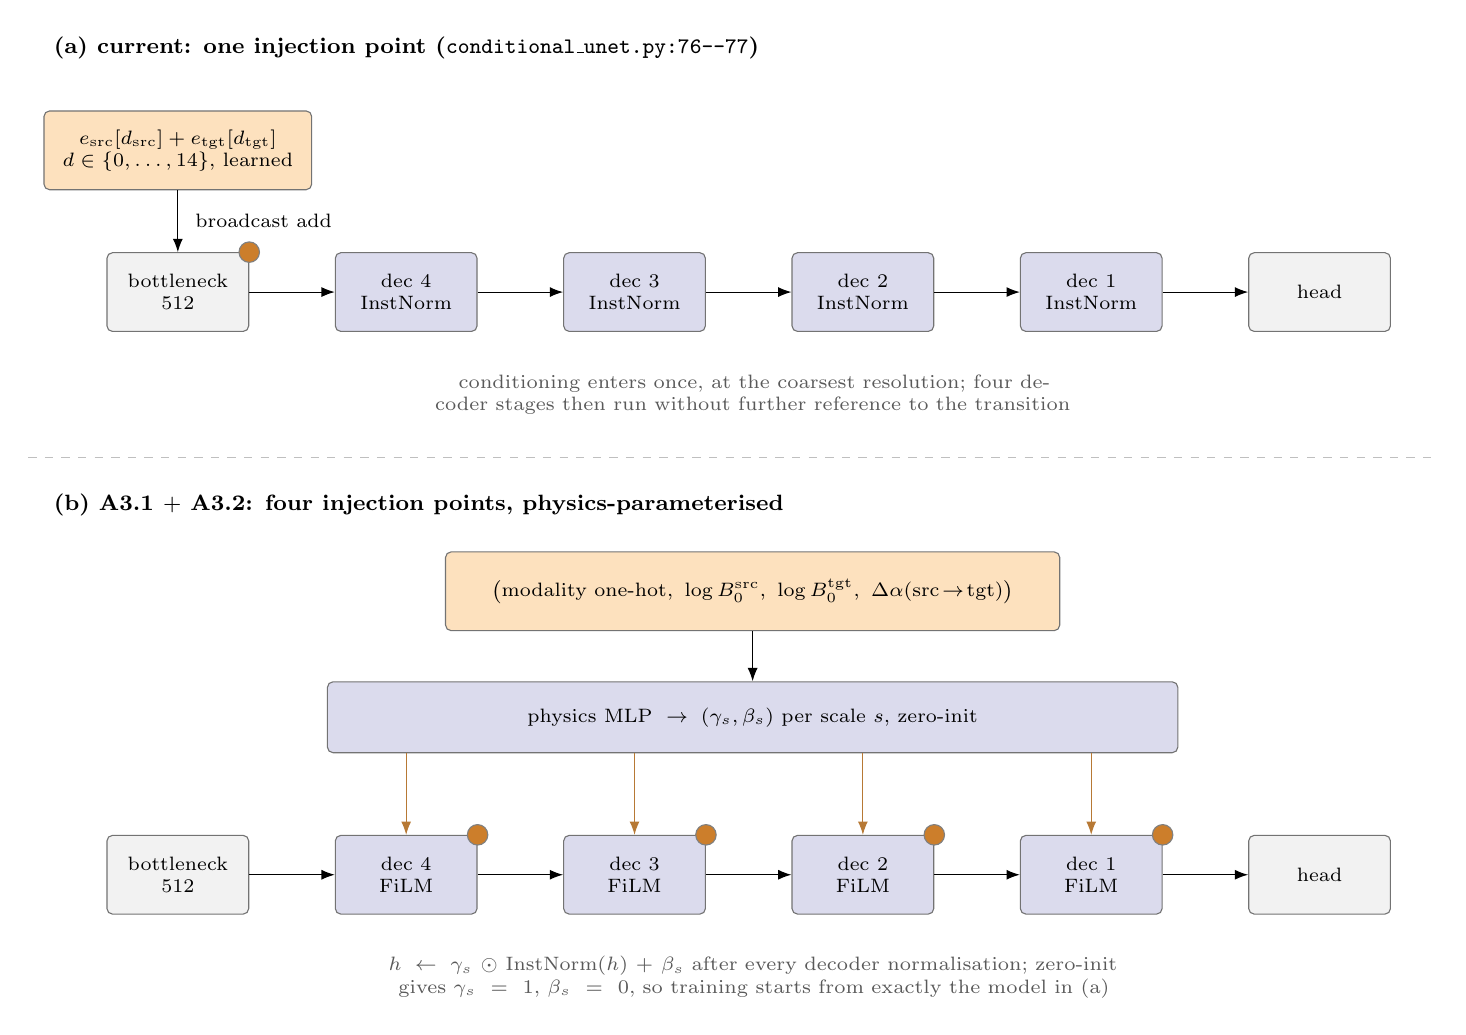
\begin{tikzpicture}[
    >=Latex,
    font=\small,
    blk/.style={draw=black!55, rounded corners=2pt, minimum height=10mm, align=center, font=\scriptsize},
    gen/.style={blk, fill=black!5},
    act/.style={blk, fill=BurntOrange!22},
    net/.style={blk, fill=NavyBlue!14},
    inj/.style={circle, fill=BurntOrange!80!black, draw=black!50, minimum size=2.6mm, inner sep=0pt},
  ]
    % ---------- (a) current ----------
    \node[font=\bfseries\footnotesize, anchor=west] at (-0.7,2.5)
      {(a) current: one injection point (\texttt{conditional\_unet.py:76--77})};

    \node[act, minimum width=34mm] (emb) at (1.0,1.2)
      {$e_{\mathrm{src}}[d_{\mathrm{src}}] + e_{\mathrm{tgt}}[d_{\mathrm{tgt}}]$\\
       $d \in \{0,\dots,14\}$, learned};

    \node[gen, minimum width=18mm] (bn) at (1.0,-0.6)  {bottleneck\\$512$};
    \node[net, minimum width=18mm] (d4) at (3.9,-0.6)  {dec 4\\InstNorm};
    \node[net, minimum width=18mm] (d3) at (6.8,-0.6)  {dec 3\\InstNorm};
    \node[net, minimum width=18mm] (d2) at (9.7,-0.6)  {dec 2\\InstNorm};
    \node[net, minimum width=18mm] (d1) at (12.6,-0.6) {dec 1\\InstNorm};
    \node[gen, minimum width=18mm] (hd) at (15.5,-0.6) {head};
    \foreach \a/\b in {bn/d4, d4/d3, d3/d2, d2/d1, d1/hd} \draw[->] (\a) -- (\b);
    \draw[->] (emb) -- node[right, font=\scriptsize, xshift=1mm] {broadcast add} (bn);
    \node[inj] at (bn.north east) {};
    \node[font=\scriptsize, align=center, text width=95mm, black!65] at (8.3,-1.9)
      {conditioning enters once, at the coarsest resolution; four decoder stages then run
       without further reference to the transition};

    \draw[black!25, dashed] (-0.9,-2.7) -- (17.0,-2.7);

    % ---------- (b) proposed ----------
    \node[font=\bfseries\footnotesize, anchor=west] at (-0.7,-3.3)
      {(b) A3.1 $+$ A3.2: four injection points, physics-parameterised};

    \node[act, minimum width=78mm] (feat) at (8.3,-4.4)
      {$\big(\text{modality one-hot},\ \log B_0^{\mathrm{src}},\ \log B_0^{\mathrm{tgt}},\
        \Delta\alpha(\mathrm{src}\!\to\!\mathrm{tgt})\big)$};
    \node[net, minimum width=108mm, minimum height=9mm] (mlp) at (8.3,-6.0)
      {physics MLP $\;\to\;(\gamma_s, \beta_s)$ per scale $s$, zero-init};
    \draw[->] (feat) -- (mlp);

    \node[gen, minimum width=18mm] (bn2) at (1.0,-8.0)  {bottleneck\\$512$};
    \node[net, minimum width=18mm] (e4)  at (3.9,-8.0)  {dec 4\\FiLM};
    \node[net, minimum width=18mm] (e3)  at (6.8,-8.0)  {dec 3\\FiLM};
    \node[net, minimum width=18mm] (e2)  at (9.7,-8.0)  {dec 2\\FiLM};
    \node[net, minimum width=18mm] (e1)  at (12.6,-8.0) {dec 1\\FiLM};
    \node[gen, minimum width=18mm] (hd2) at (15.5,-8.0) {head};
    \foreach \a/\b in {bn2/e4, e4/e3, e3/e2, e2/e1, e1/hd2} \draw[->] (\a) -- (\b);
    \foreach \n in {e4,e3,e2,e1} {
      \draw[->, BurntOrange!70!black] (mlp.south -| \n) -- (\n.north);
      \node[inj] at (\n.north east) {};
    }
    \node[font=\scriptsize, align=center, text width=105mm, black!65] at (8.3,-9.3)
      {$h \leftarrow \gamma_s \odot \mathrm{InstNorm}(h) + \beta_s$ after every decoder normalisation;
       zero-init gives $\gamma_s = 1$, $\beta_s = 0$, so training starts from exactly the model in (a)};
  \end{tikzpicture}}
  \caption{A3.1 and A3.2. The change is not more capacity but more places for the transition to act, and
  a parameterisation in which the twenty transitions share structure. Conditioning is the one lever the
  log credits with a large effect (\num{0.8699} to \num{0.8976} SSIM), and (a) shows how little of the
  network it currently reaches. The tubelet translator already implements (b)'s left half --- per-stage
  zero-initialised FiLM at all four decoder stages, conditioned on three separate embeddings rather than
  one fifteen-way index (\texttt{tubelet\_model.py:131--135, 172--173}).}
  \label{fig:film}
\end{figure}

\subsection{A4 --- Tasks 1 and 2, where nobody is competing}
\label{sec:A4}

Tasks~1 and~2 are scored on \emph{five} metrics; Task~3 on three. Almost all recent effort has gone to
Task~3. Finding~F1 is why that is a mistake: on Task~1 the identity control has the highest Dice of any
model in the log, \num{0.8549} against CUT's \num{0.8542} and CycleGAN's \num{0.8498}, and its volume
consistency is within \num{0.002} of the best. Two of five ranked metrics are being scored and not
competed for.

\paragraph{A4.1.} Apply the A2 calibration map to the Task~1 and Task~2 inputs and submit. Because the
map is monotone per (modality, source, target) it moves intensities without moving boundaries, so the
expectation is Dice and volume consistency near identity level with \rmse{} improved.

\paragraph{A4.2.} Run \texttt{scripts/segment\_predictions.py} on the result and confirm Dice and volume
consistency locally before spending a submission slot. This needs the TensorFlow environment used by
\texttt{Evaluation/segment.py}, not the \texttt{mri} environment.
\fals If the calibrated output's Dice falls below the identity's \num{0.8549}, a monotone intensity map
is not label-preserving in SynthSeg's~\cite{billot2023synthseg} eyes and the premise of A4 fails. A4.2
exists so that this is discovered locally rather than on the leaderboard.

\subsection{A5 --- encoder transfer, promoted to a first-class experiment}
\label{sec:A5}

The model we were about to build by hand already exists. \texttt{ConditionalTubeletTranslator}
(\texttt{lejepa\_pretraining/repo/mrixfields\_downstream/tubelet\_model.py}) \emph{is} ``LeJEPA encoder
$+$ conditioned U-Net'', and it already contains both changes A1.1 and A3.1 propose for the 2D model:
per-stage zero-initialised FiLM, with $(\gamma, \beta)$ read off
\texttt{condition\_projections[stage]} and applied as \texttt{value * (1 + gamma) + beta} at all four
decoder stages, weight and bias zero-initialised (\texttt{tubelet\_model.py:131--135, 172--173}); and a
zero-initialised residual head in logit space. It has only ever been run for two epochs, with no control.

\paragraph{A5.1 (done).} The artifact is pulled and checked: \num{86.66}\,M parameters, schema~v2, step
\num{40000} of a planned \num{90000}, strict load verified, all four provenance hashes matching
\texttt{run\_metadata.json}. The file is
\texttt{lejepa\_pretraining/artifacts/encoder\_step\_00040000.pt}.

\paragraph{A5.2 --- the matched control.} Same Tubelet-UNETR, same leave-one-subject-out fold, same
10-epoch budget as the current leader, two arms: LeJEPA initialisation against random initialisation.
This settles the encoder question and is the paper's central result; Furkan's design record names it as
the one omission. \emph{On priority:} at a matched two-epoch budget the encoder wins \rmse{}
(\num{0.2383} against \num{0.2436}) and LPIPS (\num{0.0889} against \num{0.0967}) but loses SSIM
(\num{0.8893} against \num{0.8942}). Since SSIM is the ranked metric this is no longer the first
experiment --- it sits at days~5--9, after the free SSIM has been taken --- but \num{0.0049} is inside
the unmeasured seed spread, so it is not settled against the encoder either.
\fals If random initialisation beats LeJEPA initialisation on held-out SSIM at a matched 10-epoch budget
by more than the A0.3 seed floor, the pretrained encoder does not transfer at this scale, and B1's
positive control becomes the only remaining reason to continue with it.

\paragraph{A5.3 --- extend the winning arm to the leader's budget} and submit if it beats
\num{0.9026} / \num{0.2329} / \num{0.0816}.

\section{The tubelet encoder measurement}
\label{sec:tubelet}

\reporttwo{} described the tubelet-ViT LeJEPA encoder~\cite{lejepa}, reported that pretraining was stable,
made \emph{no} transfer claim, and named the open risk in one sentence: the objective is computed on the
pooled CLS path while the downstream translator consumes dense tokens, and \emph{``the gap between those
two paths is the design's main open risk''}. The three-part validation was listed as unrun. It has in
fact been run. The numbers below are from
\texttt{lejepa\_pretraining/\allowbreak artifacts/\allowbreak monitor\_step\_00040000.json}, pulled from the run folder on
2026-09-05, at global step \num{40000}, on the first global view; the monitor reports all quantities
finite and its own pass flag true.

Throughout, effective rank is
\begin{equation}
  \mathrm{Rank}_{\mathrm{eff}}(Z) = \exp\Big(-\sum_k p_k \log p_k\Big),
  \qquad p_k = \sigma_k \Big/ \sum_j \sigma_j,
  \label{eq:erank}
\end{equation}
the exponentiated entropy of the normalised singular spectrum of the feature matrix $Z$: the number of
directions the representation actually uses. It is bounded by $\min(N, D)$, so the CLS statistic over
\num{300} base slabs is capped at \num{299} and the dense statistic over $768$-dimensional tokens at
\num{768}. All deltas are against the same monitor run at step~0, i.e.\ against the identical
architecture at random initialisation.

\begin{table}[H]
  \centering
  \small
  \caption{Tubelet encoder monitor at step \num{40000}, global view~0, against the same monitor at
  step~0. Retrieval is top-1 nearest-neighbour from the first global view to each of the other seven
  views of the same slab, over \num{300} slabs; dense statistics are over the \num{1568} tokens of each
  of \num{60} slabs, with effective rank computed per slab and then aggregated. Correspondence compares
  the token at a tubelet coordinate against the token at the same coordinate in a second view (matched),
  at a different coordinate in the same subject, and in a different subject; its mean coverage is
  \num{0.6659}.}
  \label{tab:cls}
  \begin{tabular}{lcc}
    \toprule
    & value & $\Delta$ vs.\ step 0 \\
    \midrule
    \multicolumn{3}{l}{\emph{CLS path --- what the loss is computed on}} \\
    \quad CLS effective rank (max \num{299}) & 95.70 & \best{$+66.00$} \\
    \quad CLS scale & 0.2567 & $-0.0044$ \\
    \quad Retrieval top-1, global $\to$ global (view $0\!\to\!1$) & 0.9833 & \best{$+0.4567$} \\
    \quad Retrieval top-1, global $\to$ local (views $0\!\to\!2\dots7$) & 0.8833--0.9100 &
      \best{$+0.59$ to $+0.65$} \\
    \midrule
    \multicolumn{3}{l}{\emph{Dense path, final layer --- see Section~\ref{sec:scope}}} \\
    \quad Dense effective rank, mean (max \num{768}) & 115.06 & \best{$-69.98$} \\
    \quad Dense effective rank, min & 96.07 & $-41.37$ \\
    \quad Dense scale, mean & 0.2141 & $-0.0780$ \\
    \midrule
    \multicolumn{3}{l}{\emph{Coordinate-matched correspondence, final layer} (cosine)} \\
    \quad matched location, matched subject & 0.9734 & $+0.0008$ \\
    \quad wrong location, same subject & 0.9556 & $-0.0096$ \\
    \quad wrong subject & 0.9415 & $-0.0052$ \\
    \quad \textbf{matched $-$ wrong-location gap} & \best{0.0177} & $+0.0103$ \\
    \quad matched $-$ wrong-subject gap & 0.0320 & $+0.0060$ \\
    \bottomrule
  \end{tabular}
\end{table}

\paragraph{The CLS path --- what the loss trains --- is healthy.} No collapse, and a large genuine gain
in view-invariant slab identity over a random ViT: \num{66} points of effective rank, and a local
$8\times96\times96$ sub-slab retrieves its parent global view roughly nine times in ten against one time
in four at initialisation. The objective is optimising what it was written to optimise.

\paragraph{The final-layer dense tokens are worse than random initialisation.} They have lost \num{70}
points of effective rank, and the correspondence block of Table~\ref{tab:cls} shows what that costs. Every such token sits at cosine
$\approx 0.94$--$0.97$ with every other one regardless of anatomy. Features whose job is to say
\emph{where} they are separate the right location from a wrong one by \num{0.0177} of cosine, and
\num{40000} steps of training have widened that separation by only \num{0.0103}. The two facts are
consistent with each other and with the objective: Equation~\ref{eq:erank} falls when the representation
concentrates into fewer directions, and a loss that rewards only view-invariant pooled identity has no
term that penalises tokens for becoming interchangeable.

\subsection{What the monitor does not measure}
\label{sec:scope}

The monitor's \texttt{encode\_monitor\_views} calls \texttt{encoder.forward\_tokens}
(\texttt{mrixfields\_lejepa/\allowbreak tubelet\_training.py:473--492}), which returns the \emph{final-layer},
post-LayerNorm token grid. The translator does not consume that grid. It calls
\texttt{forward\_intermediate\_tokens} with the default \texttt{indices=(2,5,8,11)}
(\texttt{mrixfields\_lejepa/\allowbreak tubelet\_encoder.py:228--232}) and uses the four returned grids as
\texttt{block3, block6, block9, block12} for its skip connections and bottleneck
(\texttt{tubelet\_model.py:209}). \textbf{Three of the four grids the decoder actually eats have never
been measured}, and the one that has is not among them.

Two consequences. The measurement above is evidence that the \emph{final layer} degrades under a
CLS-only objective; it is not evidence that the encoder carries nothing usable downstream, and the
earlier reading --- that the risk had materialised and encoder transfer should therefore be dropped ---
does not follow from it. And the obvious follow-up is one monitor change rather than one training run:
extend the diagnostics to blocks 2, 5, 8 and 11. That also answers a question we would otherwise guess
at, namely which depth the translator should tap.

\paragraph{The leaderboard pair is a budget confound, not a tax.} The tubelet row in
Table~\ref{tab:position} is a \emph{two-epoch} run --- the design record specifies ``fine-tune the
complete encoder for two epochs'' (\texttt{docs/conditional\_tubelet\_translator\_design.md:28}) ---
while the \num{0.9026} row is ten epochs. Against the matched two-epoch scratch 3D U-Net, the LeJEPA
initialisation wins \rmse{} (\num{0.2383} against \num{0.2436}) and LPIPS (\num{0.0889} against
\num{0.0967}) and loses SSIM by \num{0.0049} (\num{0.8893} against \num{0.8942}) --- a margin inside the
seed spread that A0.3 has not yet measured. The comparison is unresolved in both directions, which is
exactly what A5.2 is for.

\paragraph{What follows for the paper.} B1 keeps the finding at the scope the evidence supports:
\emph{a CLS-only LeJEPA objective can improve pooled representation quality substantially while
degrading final-layer dense token quality below random initialisation.} Two cheap controls make it
publishable: the depth sweep above, and a coordinate-level token term alongside the CLS objective, which
is one training run.

\begin{figure}[t]
  \centering
  \resizebox{0.76\linewidth}{!}{%
  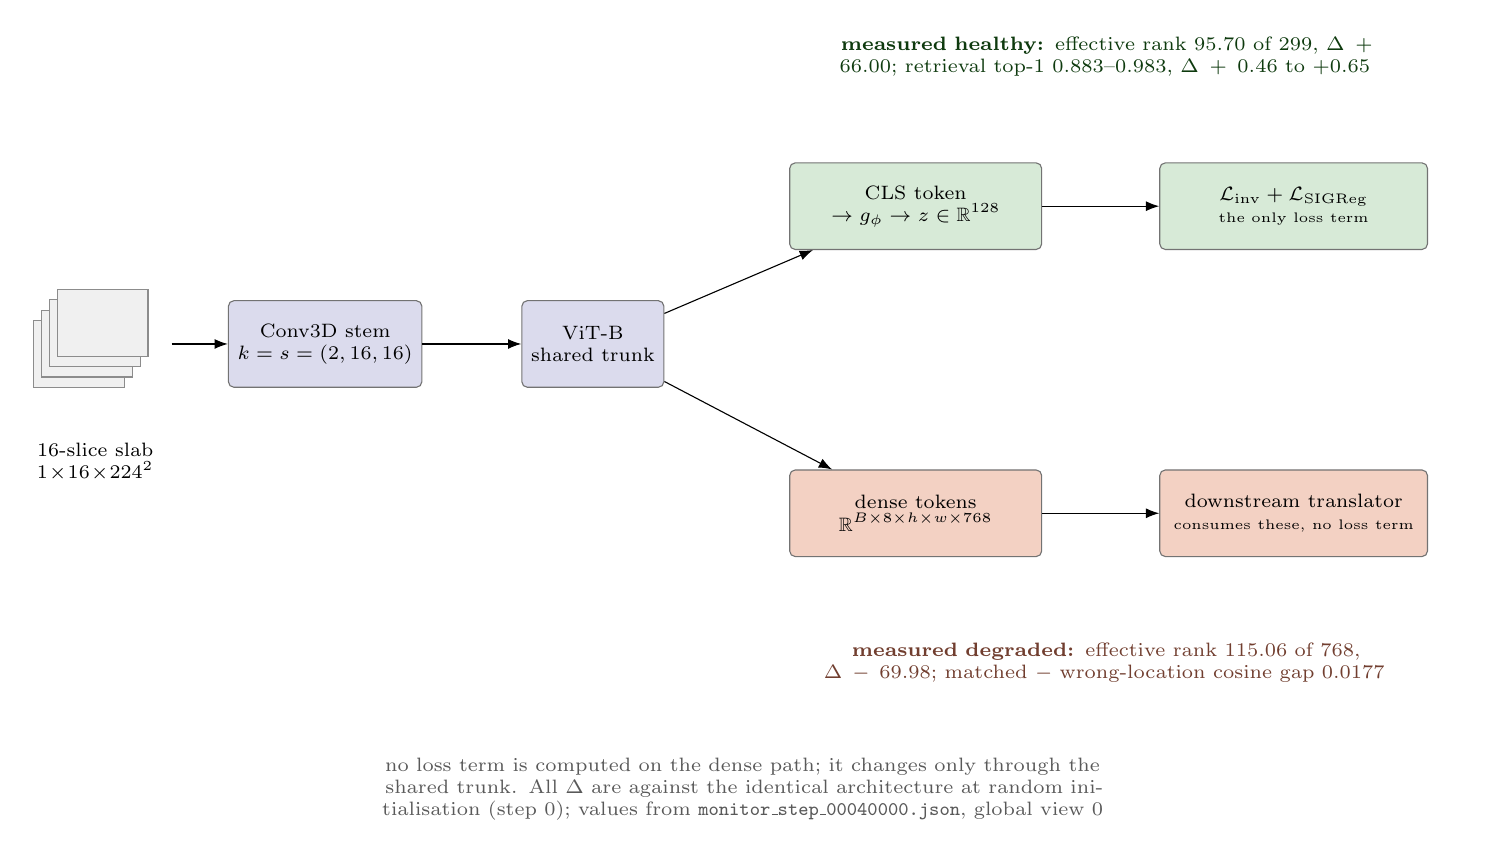
\begin{tikzpicture}[
    >=Latex,
    font=\small,
    blk/.style={draw=black!55, rounded corners=2pt, minimum height=11mm, align=center, font=\scriptsize},
    gen/.style={blk, fill=black!5},
    net/.style={blk, fill=NavyBlue!14},
    ok/.style={blk, fill=ForestGreen!18},
    bad/.style={blk, fill=BrickRed!16},
  ]
    \foreach \i in {0,1,2,3}
      \draw[draw=black!45, fill=black!6] (0.10*\i, 0.13*\i) rectangle ++(1.15,0.85);
    \node[font=\scriptsize, align=center] at (0.78,-0.95) {16-slice slab\\$1\!\times\!16\!\times\!224^2$};

    \node[net, minimum width=24mm] (stem) at (3.7,0.55) {Conv3D stem\\$k=s=(2,16,16)$};
    \node[net, minimum width=18mm] (vit)  at (7.1,0.55) {ViT-B\\shared trunk};

    \node[ok,  minimum width=32mm] (cls)   at (11.2,2.3)  {CLS token\\$\to g_\phi \to z \in \mathbb{R}^{128}$};
    \node[ok,  minimum width=34mm] (loss)  at (16.0,2.3)
      {$\mathcal{L}_{\mathrm{inv}} + \mathcal{L}_{\mathrm{SIGReg}}$\\{\tiny the only loss term}};
    \node[bad, minimum width=32mm] (dense) at (11.2,-1.6) {dense tokens\\$\mathbb{R}^{B\times 8\times h\times w\times 768}$};
    \node[bad, minimum width=34mm] (down)  at (16.0,-1.6)
      {downstream translator\\{\tiny consumes these, no loss term}};

    \draw[->] (1.75,0.55) -- (stem);
    \draw[->] (stem) -- (vit);
    \draw[->] (vit) -- (cls);
    \draw[->] (vit) -- (dense);
    \draw[->] (cls) -- (loss);
    \draw[->] (dense) -- (down);

    \node[font=\scriptsize, align=center, text width=92mm, ForestGreen!42!black] at (13.6,4.2)
      {\textbf{measured healthy:} effective rank $95.70$ of $299$, $\Delta +66.00$;
       retrieval top-1 $0.883$--$0.983$, $\Delta +0.46$ to $+0.65$};
    \node[font=\scriptsize, align=center, text width=92mm, BrickRed!52!black] at (13.6,-3.5)
      {\textbf{measured degraded:} effective rank $115.06$ of $768$, $\Delta -69.98$;
       matched $-$ wrong-location cosine gap $0.0177$};

    \node[font=\scriptsize, align=center, text width=118mm, black!65] at (9.0,-5.1)
      {no loss term is computed on the dense path; it changes only through the shared trunk.
       All $\Delta$ are against the identical architecture at random initialisation (step 0);
       values from \texttt{monitor\_step\_00040000.json}, global view 0};
  \end{tikzpicture}}
  \caption{The CLS/dense split, \emph{at the depth the monitor measures}. One trunk, two output paths,
  and a loss attached to exactly one of them. After \num{40000} steps the supervised path has gained
  \num{66} points of effective rank and become strongly view-invariant, while the final-layer dense
  tokens have lost \num{70} and barely distinguish a matched anatomical location from a wrong one. The
  translator does not read this layer: it taps blocks 2, 5, 8 and 11, three of which have never been
  measured (Section~\ref{sec:scope}). The figure bounds what is known, not what transfers.}
  \label{fig:clsdense}
\end{figure}

\section{Horizon B --- fastMRI and a paper}
\label{sec:horizonB}

Ordered by how much of each item is already in hand.

\paragraph{B1 --- the dense/CLS gap in tubelet LeJEPA.} Section~\ref{sec:tubelet}. The negative result is
measured at the final layer; what remains is the depth sweep of Section~\ref{sec:scope}, the positive
control (a coordinate-level dense term added to the CLS objective, one training run), and the causal
transfer test of A5.2. The claim is architecture-independent: it is a statement about what a pooled-only
objective does to dense tokens, not about MRI.

\paragraph{B2 --- synthetic pretraining transfer test.} The corrected generator reaches between-volume
diversity ratios of \numrange{0.86}{0.98} at \SI{0.1}{\tesla}, \SI{3}{\tesla} and \SI{5}{\tesla}, with
\SI{1.5}{\tesla} still short at \num{0.65}, but nothing has been pretrained on it, so the premise ---
that synthetic pairs transfer, the Image Quality Transfer setup~\cite{alexander2017iqt} --- is untested.
Run the $2\times2$ over $\{\text{random}, \text{pretrained}\}$ and
$\{\text{real pairs}, \text{synthetic} \to \text{real}\}$, with the A2 control as a fifth row so the
outcome reads as ``moved from below the zero-parameter baseline to above it''.

\paragraph{B3 --- rebuild the generator on SynthSeg's own machinery.} Per-label GMM statistics from
\texttt{estimate\_priors.build\_intensity\_stats} cover roughly \num{32} disjoint labels instead of the
three soft tissues used today, which removes the over-summing term in \reporttwo{}'s remap outright,
since hard labels cannot over-sum. \texttt{BrainGenerator} adds bias field, slice-thickness and
anisotropic-resolution simulation and nonlinear deformation, none of which the current four-step operator
models at all~\cite{billot2023synthseg}. Per-sample per-label sampling should also fix the
\SI{1.5}{\tesla} diversity shortfall structurally rather than by tuning.

\paragraph{B4 --- a contrast-agnostic perceptual loss.} The LPIPS term uses AlexNet features trained on
natural photographs. SynthSeg's encoder was trained to be invariant to MRI contrast and resolution, which
is exactly the invariance a field-translation perceptual metric needs. Distil it into a small 3D U-Net
--- its own generator supplies unlimited training data --- freeze it, and use its features. That also
supplies the differentiable segmenter a Dice or volume-consistency term on Tasks~1 and~2 would need.

\paragraph{B5 --- spectral-profile loss.} Penalise
$\lvert \log P_{\mathrm{pred}}(f) - \log P_{\mathrm{tgt}}(f)\rvert$ over the \numrange{0.02}{0.20} fit
band instead of hand-set band weights. This optimises the exact quantity \reportone{} measured and gets
the sign right by construction at every transition, which a fixed $w_b$ of the UniField kind~\cite{lin2026unifield} cannot. \reporttwo{} argued that
from a nine-entry table; on the full grid the case is sharper, since exactly \num{30} of the
\num{60} transition-by-modality $\Delta\alpha$ cells in \texttt{reports/spectral/alpha\_summary.csv} are
negative. A transition-independent, fixed-sign band weighting therefore has the wrong sign for precisely
half the cells, which is the argument for a profile loss over hand-derived signed weights.
\texttt{scripts/spectral\_analysis.py} already has the RAPSD machinery.

\paragraph{B6 --- port to fastMRI.} Three travelling-volunteer subjects is the binding constraint on
every claim here, the seed-floor problem of A0.3 included. fastMRI expands the study past it, and makes
B1's result testable where the effect separates from subject identity.

\section{Schedule and status}
\label{sec:schedule}

\begin{table}[H]
  \centering
  \small
  \caption{Suggested order. Days~6--9 run in parallel: different task, different person.}
  \label{tab:schedule}
  \begin{tabular}{llp{8.0cm}}
    \toprule
    When & What & Why \\
    \midrule
    Days 1--2 & A0.1, A0.5 & The held-out fold, then the six-checkpoint sweep. No training. Tests
      whether six weeks of architecture search has been reading checkpoint noise. \\[2pt]
    Days 2--3 & A0.3, A1.2, A1.3 & Seed floor, dihedral TTA and checkpoint averaging --- all three act on
      SSIM, none needs a new architecture. \\[2pt]
    Days 3--4 & A2 & Zero-parameter calibration control. Its SSIM effect is unmeasured, unlike its
      \rmse{} effect, so one cheap submission rather than a threat to the leader. \\[2pt]
    Days 4--7 & A3 & Conditioning is still the only large measured effect on SSIM
      (\num{0.8699} to \num{0.8976}). \\[2pt]
    Days 5--9 & A5.2 & The matched encoder control. Demoted from first because the encoder is
      \num{0.0049} SSIM behind scratch at matched two epochs; still the paper's core result. \\[2pt]
    Days 6--9 & A4 & Different task, different person, in parallel. Clearest unclaimed rank-sum win. \\[2pt]
    Days 9--12 & \multicolumn{2}{l}{Submissions, freeze, write up} \\
    \midrule
    After & B1 $\to$ B2 $\to$ B4 & B1 needs the depth sweep and the positive control. \\
    \bottomrule
  \end{tabular}
\end{table}

\paragraph{Status, 2026-09-05.} {\sloppy\hbadness=10000 The combined model is implemented and training. The tubelet
translator is wired into this pipeline by a new registered component,
\texttt{components/models/conditional\_tubelet.py}, driven by the configuration
\texttt{experiment-pipeline/configs/task3\_tubelet\_pro.toml}: $16 \times 224 \times 224$ slabs at batch
4 for ten epochs, with a real validation split (\texttt{holdout\_subjects = ["0009"]},
\texttt{early\_stopping\_monitor = "validation"}).\par} It is the first
Task~3 run in the project with a real held-out subject, and it is the A5.2 arm. Measured cost:
\SI{12.8}{\gibi\byte} on the \SI{32}{\giga\byte} GV100, about \num{1.7} batches per second, about two
minutes per epoch.

\paragraph{Open items that can move the schedule.} Three, none of them research. Confirm with Furkan
whether the pretraining run is finished, stalled or still going --- the newest export is step
\num{40000}, the config targets \num{90000} and \texttt{run\_metadata.json} records
\texttt{stop\_after\_steps: 60000} --- since B1 needs to know which. Decide between
\texttt{make\_task3\_submission.py} and \texttt{scripts/generate\_challenge\_submission.py}, which cannot
run at all: its \texttt{validate\_inputs()} requires an \texttt{official/MRIxFields2026/} checkout absent
from this repository. And pick one MLflow root: tracking URIs are cwd-relative and runs have been
launched from two.

\begin{thebibliography}{99}
\small

\bibitem{report1}
B.~D. Kahya, F.~Yüceyalç\i{}n, R.~Badreddine, A.~Zelka. \emph{MRIxFields 2026: Progress Report --- Baselines,
Representation Learning, and a Spectral View of Field-Strength Translation}. Internal project report,
2026.

\bibitem{lin2026unifield}
Y.~Lin, C.~Wang, Z.~Peng, Y.~Yuan. \emph{UniField: A Unified Field-Aware MRI Enhancement Framework}.
MICCAI, 2026. \url{https://arxiv.org/abs/2603.09223}

\bibitem{meng2025fpsformer}
Y.~Meng, Z.~Yang, Y.~Shi, Z.~Song. \emph{Boosting ViT-based MRI Reconstruction from the Perspectives of
Frequency Modulation, Spatial Purification, and Scale Diversification}. AAAI, 2025.
\url{https://arxiv.org/abs/2412.10776}

\bibitem{alexander2017iqt}
D.~C. Alexander et al. \emph{Image quality transfer and applications in diffusion MRI}. NeuroImage, 2017.

\bibitem{billot2023synthseg}
B.~Billot et al. \emph{SynthSeg: Segmentation of brain MRI scans of any contrast and resolution without
retraining}. Medical Image Analysis, 2023.

\bibitem{lejepa}
R.~Balestriero, Y.~LeCun. \emph{LeJEPA: Provable and Scalable Self-Supervised Learning Without the
Heuristics}, 2025. \url{https://arxiv.org/abs/2511.08544}

\end{thebibliography}

\end{document}
